\begin{figure}[h]\centering
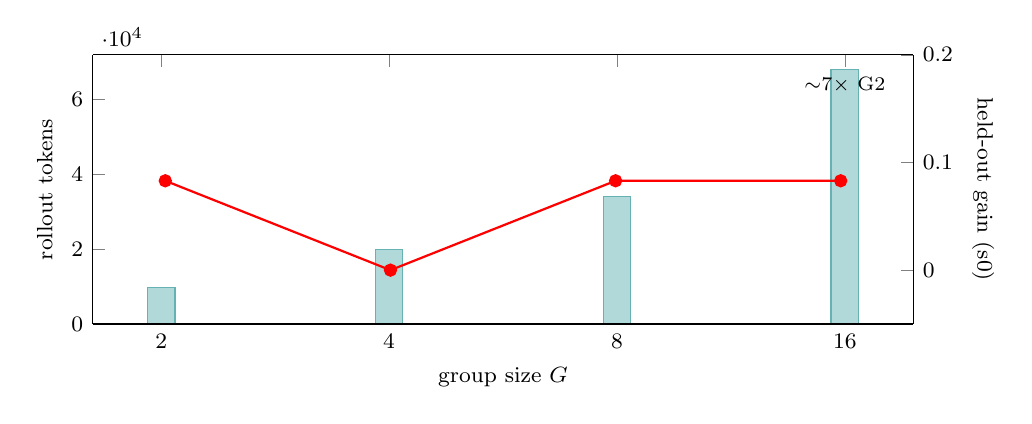
\begin{tikzpicture}
\begin{axis}[width=12cm,height=5cm,
  xlabel={group size $G$},ylabel={rollout tokens},
  xmode=log,log basis x=2,xtick={2,4,8,16},xticklabels={2,4,8,16},
  ymin=0,ymax=72000,tick label style={font=\footnotesize},label style={font=\footnotesize},
  axis y line*=left]
\addplot[fill=teal!30,draw=teal!60,ybar,bar width=10pt] coordinates {(2,9663)(4,19964)(8,34084)(16,68055)};
\node[font=\scriptsize] at (axis cs:16,64000){$\sim$7$\times$ G2};
\end{axis}
\begin{axis}[width=12cm,height=5cm,xmode=log,log basis x=2,xmin=1.6,xmax=20,
  ymin=-0.05,ymax=0.2,axis y line*=right,ylabel={held-out gain (s0)},
  xtick=\empty,tick label style={font=\footnotesize},label style={font=\footnotesize},
  y label style={rotate=180}]
\addplot[red,mark=*,thick] coordinates {(2,0.083)(4,0.0)(8,0.083)(16,0.083)};
\end{axis}
\end{tikzpicture}
\caption{P3 group size (real data, seed 0). Rollout tokens (bars) scale $\sim$linearly with $G$ (G16 $\approx7\times$ G2); held-out gain (red) shows \emph{no robust sweet spot} --- G4 was in fact the weakest single point. The earlier single-seed ``G=4 sweet spot'' claim does not survive.}
\end{figure}
